The program is intended to help with evaluation of the many index expressions
which arise in multi-reference pertrbation theory.  Essentially, it aims to
evaluate one of the follwing three kinds of expressions, the simplest of which
is
\begin{equation}
\langle M | \hat{X} \hat{Y} ... | N \rangle,
\label{eqn:basic}
\end{equation}
\noindent here $\hat{X}$ and $\hat{Y}$ are some arbitrary operators, and $| N
\rangle$  is a multireference wavefunction represented as a linear combination
of determinants, $|I\rangle $;
\begin{equation}
|N\rangle = \sum_{I} c_{I}^{N}| I \rangle.
\end{equation} 
\noindent There are three main types of terms the program can calculate. The simplest is :
\begin{equation}
\sum_{\substack{ x_{1}x_{2}...\\ y_{1}y_{2}... \\ ...}} X_{x_{1}x_{2}...} Y_{y_{1}y_{2}...} ...
\sum_{I}\sum_{J}
\langle I | a^{\dagger}_{x_{1}} a_{x_{2}}...a^{\dagger}_{y_{1}}a_{y_{2}}....| J \rangle 
 c^{M \dagger}_{I}c^{N}_{J}
\label{eqn:basic_2nd_quantized}
\end{equation}
\noindent  Which is just (\ref{eqn:basic}) written using second quantization;
$X_{x_{1},x_{2}...}$ is a representation of operator $\hat{X}$ in a basis of
molecular orbitals. \\

\noindent It is also possible to calculate derivatives of (\ref{eqn:basic_2nd_quantized})  with respect to ci-coefficients, $c_{I}^{N}$;
\begin{equation}
\sum_{\substack{ x_{1}x_{2}...\\ y_{1}y_{2}... \\ ...}} X_{x_{1}x_{2}...} Y_{y_{1}y_{2}...} ...
\sum_{J}
\langle I | a^{\dagger}_{x_{1}} a_{x_{2}}...a^{\dagger}_{y_{1}}a_{y_{2}}....| J \rangle 
c^{N}_{J}
\label{eqn:ci_derivative}
\end{equation}
\noindent In a simlar vein, it is possible to expressions of form:
\begin{equation*}
\sum_{\substack{ x_{1}x_{2}...\\ y_{1}y_{2}... \\ ...}} X_{x_{1}x_{2}...} Y_{y_{1}y_{2}...} ...
\sum_{\Omega}
\sum_{I}\sum_{J}
\langle I | \hat{E}^{\dagger}_{\Omega} a^{\dagger}_{x_{1}} a_{x_{2}}...a^{\dagger}_{y_{1}}a_{y_{2}}....| J \rangle 
 c^{M \dagger}_{I}c^{N}_{J}
\end{equation*}
\begin{equation}
=
\sum_{\substack{ x_{1}x_{2}...\\ y_{1}y_{2}... \\ ...}} X_{x_{1}x_{2}...} Y_{y_{1}y_{2}...} ...
\sum_{I}\sum_{J}
\langle I | a_{\omega_{1}} a_{\omega_{2}}.. .a^{\dagger}_{x_{1}} a_{x_{2}}...a^{\dagger}_{y_{1}}a_{y_{2}}....| J \rangle 
 c^{M \dagger}_{I}c^{N}_{J}
\label{eqn:basic_2nd_quantized_projector}
\end{equation}
\noindent where the $\hat{E}^{\dagger}_{\Omega}$ is an projection operator
which excites electrons from the orbitals used to construct the space in which
the reference wavefunctions, $\{|N\rangle\}$, were originally defined into some
virtual space.\\

\noindent The program is intended to be flexible; and instead of asking for
specific perturbation theories or properties, the user has the option of
specifing algebraic expressions directly via the input file.

\section*{Structural outline}
\noindent The program is split into three main components; an algebraic manipulator, an FCI
and tensor contraction library, and a task manager.\\

\begin{figure}[!ht]
\begin{center}
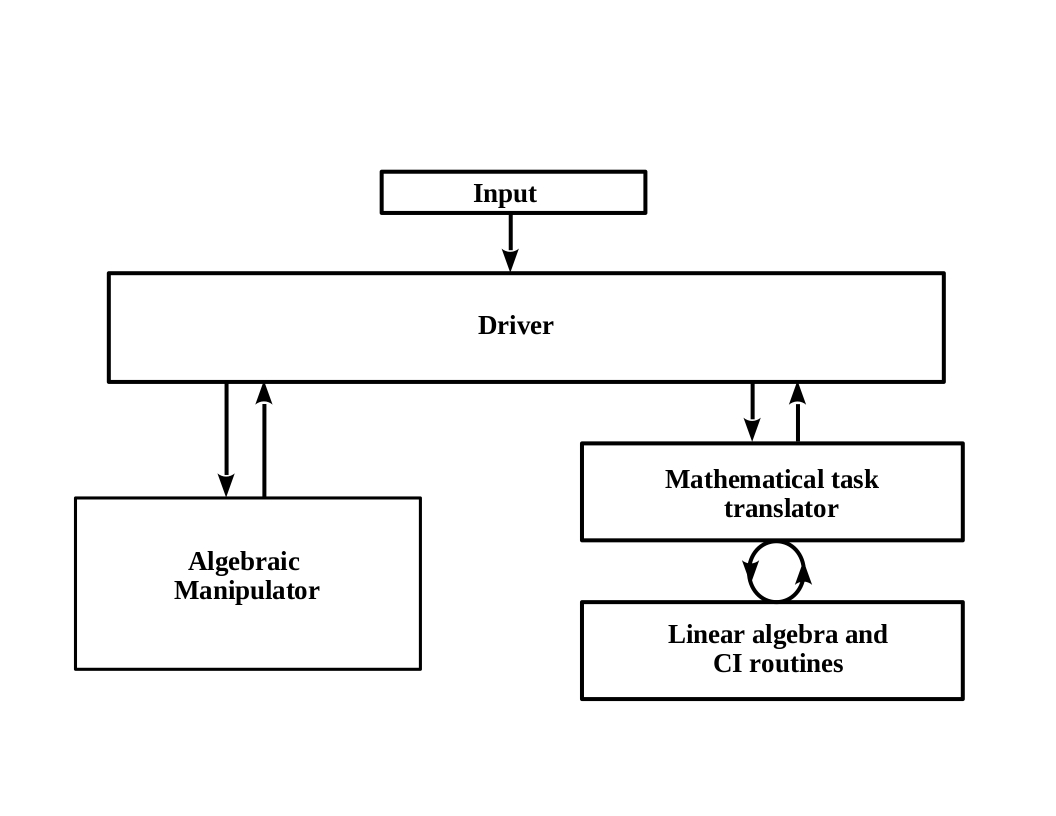
\includegraphics[width=0.8\textwidth]{prog_structure.jpg}
\caption{ Basic program structure. }
\end{center}
\label{fig:prog_structure}
\end{figure}

\noindent The algebraic manipulator interprets the expressions defined
in the input, and restructures these into a number of quantities which are
more suited to computational evaluation. To accomplish this the
algebraic manipulator makes extensive use of the commutation
relations of the creation and annihilation operators, as well as the physical
symmetries of the operators, in order to minimize the number of terms, and
avoid the need for calculation of terms which are likely to be computationally
expensive to evaluate (e.g., those with large numbers of indexes). This series
of expressions is used to form an algebraic task list; a sequence of
mathematical operations which need to be evaluated.  It is important to note
that the algebraic manipulator is entirely based around symbolic manipulation,
and does not handle any of the large data structures, e.g., civectors,
molecular orbital integral tensors, etc.. The expressions in the algebraic
task list do not in any way specify what kind of data structures need to
be used to store the quantities necessary for their evaluation.\\

\noindent The FCI and tensor libraries contain generic routines for
calculating density matrices and their derivatives, and performing tensor
contractions (and other various tensor manipulations). The tensor and FCI
library are completely disctinct from the algebraic manipulator, and operate
totally independently. The FCI library is designed such that it can calculate
density matrices (and derivatives) of arbitrary order. In a similar vein, the
tensor library can operate on tensor of arbitrary rank, with each dimension
being a different size. At present the FCI  library uses the Determinant class
defined in Bagel~\cite{BAGEL}.
The tensor libraries make use of the SMITH::Tensor class defined in Bagel,
which in turn makes use of the TiledArray~\cite{TiledArray} libraries for parallel storage of the data. 
The routines in the tensor arithmetic library are built using 
a combination of calls to LAPACK~\cite{LAPACK}, and the tensor transposition routine defined in
TiledArray\footnote{ To clarify, whilst btas has some tensor contraction routines, 
these were found to not be suitable for the current purpose, and are not used.}.\\

\noindent The final major component of the program is the task translator,
which faciliates communication between the algebraic manipulator and the 
FCI and tensor libraries. This is necessary, as
the neither the arithmetic component has now knowledge of the classes used in
the algebraic manipulator, and vice versa. Whilst this has complicated the
design slightly, it should enable greater portability, as well as making the
program substantially easier to extend and upgrade.\\ 

\noindent In a sense there is a fourth component, a driving routine, which
performs some communication between the three routines, and which deals with
input reading, and some initialization. However, whilst this component is practically
important, and not particularly small, it is rather simple, and not of
interest, so I will not discuss it significantly.

\section*{ Specific components}
The functioning of the program is best explained by example. In the following,
use of italicized words indicate that word is a class defined in the program.
The "highest level" class is the \emph{equation}, which could be something like 
find the $\hat{T}^{LN}$, for all desired values of $L$ and $N$, which satisfy 
\begin{equation}
\sum_{N} 
\langle M | \hat{E}^{\dagger}_{\Omega} (\hat{H}-\epsilon_{L}) \hat{T}^{LN} | N \rangle  +
\langle M | \hat{E}^{\dagger}_{\Omega} \hat{H} | L  \rangle = 0 \text{ \ \ \ \ } \forall \text{ \ \ }  M . 
\end{equation}
\noindent This equation for is broken down into a number of components, 
or \emph{expression}s, which can be evaluated independently:
\begin{equation}
\sum_{N} 
\langle M | \hat{E}^{\dagger}_{\Omega} (\hat{H}-\epsilon_{L}) \hat{T}^{LN} | N \rangle  +
\langle M | \hat{E}^{\dagger}_{\Omega} \hat{H} | L  \rangle  
\label{eqn:Hylleras}
\end{equation}
\noindent The \emph{equation} contains a number of \emph{expression}s, along with
information regarding how they relate to one another and the solution to the equation.
In an expression of the above type the values of $L$ and $M$  would be set, whilst the range of
summation over $N$ would be defined. Note that unlike the equation the expression
contains no information about what the expression should be equal to.
Typically, a given equation will have several similar expressions,
which only different from one another by the values of the indexes or the 
ranges of the index summation.\\

\noindent Each \emph{expression} is further broken down into a number of \emph{term}s.
\emph{Terms} differ from \emph{expressions} in that any state index summation in
in a \emph{term} applies to the entire term.
Hence (\ref{eqn:Hylleras}) cannot be represented by a single term object, and instead
requires two:
\begin{equation}
\sum_{N} 
\langle M | \hat{E}^{\dagger}_{\Omega} (\hat{H}-\epsilon_{L}) \hat{T}^{LN} | N \rangle  
\label{eqn:Hylleras1}
\end{equation}
\begin{equation}
\langle M | \hat{E}^{\dagger}_{\Omega} \hat{H} | L  \rangle  
\label{eqn:Hylleras2}
\end{equation}
\noindent Without this seperation (\ref{eqn:Hylleras2}) would be summed over $N$ times,
despite the fact $N$ does not occur. 
Whilst this constraints seems needless and annoying there are justifications for them stemming
from the strategies, to be elaborated upon later in this document, used to merge different \emph{term}s together. \\ 

\noindent Each \emph{term} is further broken down into a list of \emph{braket}s. The \emph{term} 
in (\ref{eqn:Hylleras1}) would be broken down into $2N$ \emph{brakets}: 
\begin{equation}
\langle M | \hat{E}^{\dagger}_{\Omega} \hat{H} \hat{T}^{LN} | N \rangle  
\end{equation}
\begin{equation}
\langle M | \hat{E}^{\dagger}_{\Omega} (-\epsilon_{L}) \hat{T}^{LN} | N \rangle  
\end{equation}
\noindent Within a \emph{braket} the values of all the indexes are specified.
A single \emph{braket} consists of a bra and a ket, surrounding some operator
formed from the product of an arbitrary number of other operators.  The
individual \emph{braket}s comprising a \emph{term} are never\footnote{Excepting
the situation where a \emph{term} consists of a single \emph{braket}.}
evaluated independently; the arithmetic operations to evaluate \emph{braket}s
with common bra- and ket will be merged together, provided these bra and ket
exist within the same term. Similarly, it is also possible to merge the compute
lists associated with different \emph{term}s together, though not the
\emph{term} objects themselves. However, this is not done by default, as
typically it is useful to store and evaluate \emph{term}s independently.\\

\noindent The remaining fundamental classes are the \emph{TensOps}, which contain
information regarding the second-quatized presentation of the operators, e.g.,
the tensor $\mathbf{H}$, with elements $H_{ijkl}$, where $i, j, k$ and $l$ are
molecular orbital indices. And the \emph{StatesInfo}, \emph{CIVecInfo}
classes, which contains information about which ci-sectors are used to represent the 
wavefunction, and which orbitals were used to construct these ci-sectors,  respectively.\\

\noindent The above describe components are the targets upon which the 
algebraic manipulation routines act to generate the algebraic task list.
I shall now describe the proceedure, and introduce further classes as necessary.\\

\noindent It is important to note that due to the nature of the program I shall not describe the
program in the order in which it is executed, but instead start from the simplest operations it
performs, and then gradually build up to show how these can be linked together to
generate the task lists necessary for solution of the equations.
%\section{Operator definition, formation, blocking and symmetry } 
%\textbf{Key classes:} \emph{TensOp/MultiTensOp, CtrTensorPart/CtrMultiTensorPart, RangeBlock/SplitRangeBlock}  

%\section{Braket Formation} 
%\textbf{Key classes:} \emph{Expression, BraKet, GammaGenerator, GammaInfo, StateInfo, CIVecInfo}  

%\section{Algebraic Task List generation} 
%\textbf{Key classes:} \emph{Expression, GammaGenerator, AContribInfo, CtrTensOp/CtrMultiTensOp}  

%\section{Equation solver} 
%\textbf{Key classes:} \emph{Expression, TensOp/MultiTensOp, SystemInfo, Computer classes, }  
